\documentclass[10pt,twocolumn,letterpaper]{article}

\usepackage{cvpr}
\usepackage{times}
\usepackage{epsfig}
\usepackage{graphicx}
\usepackage{amsmath}
\usepackage{amssymb}
\usepackage{graphicx}
\usepackage{subcaption}

% Include other packages here, before hyperref.

% If you comment hyperref and then uncomment it, you should delete
% egpaper.aux before re-running latex.  (Or just hit 'q' on the first latex
% run, let it finish, and you should be clear).
\usepackage[breaklinks=true,bookmarks=false]{hyperref}

\cvprfinalcopy % *** Uncomment this line for the final submission

\def\cvprPaperID{****} % *** Enter the CVPR Paper ID here
\def\httilde{\mbox{\tt\raisebox{-.5ex}{\symbol{126}}}}

% Pages are numbered in submission mode, and unnumbered in camera-ready
%\ifcvprfinal\pagestyle{empty}\fi
\setcounter{page}{4321}
\begin{document}

%%%%%%%%% TITLE
%\title{\LaTeX\ Author Guidelines for CVPR Proceedings}
\title{Crop Monitoring Tool Using CV and ML}

\author{Gideon Mpungu\\
Makerere University\\
Kampala, Uganda\\
{\tt\small mpungu.gideon@students.mak.ac.ug} 
% For a paper whose authors are all at the same institution,
% omit the following lines up until the closing ``}''.
% Additional authors and addresses can be added with ``\and'',
% just like the second author.
% To save space, use either the email address or home page, not both
%\and
%%Second Author\\
%Institution2\\
%First line of institution2 address\\
%{\tt\small secondauthor@i2.org}
}

\maketitle
%\thispagestyle{empty}

%%%%%%%%% ABSTRACT
\begin{abstract}
When we look at the integration of Computer Vision in agriculture, especially in monitoring of farms or gardens without much human intervention, the accurate identification and classification of different crop varieties and weed species becomes a rather complex task. The structural similarities among these species further complicate the task, making it a major challenge even for crop specialists like botanists. This complexity, together with the growing need for efficient garden monitoring and weed control, necessitates the development of sophisticated AI and CV models to simplify and aid in solving the problem.

The goal of this research is to develop a garden monitoring tool capable of detecting and identifying specific crops and the presence of grass (weeds). In this paper, we present the development of traditional ML models, specifically Random Forest, Decision Trees, Naive Bayes, Support Vector Machine (SVM) and a Voting Classifier ensemble model of the first three models, for precise crop and weed classification in garden settings, focusing on cassava, maize, grass, and sugarcane. We combine different feature extraction methods, including color histogram, edge detection, and key point indicators to extract a training dataset for our ML models and compare their performance to build an ensemble model from the best three performers. Results indicate that Random Forest model had the highest accuracy with our combined features, with an accuracy of 97\%, and the next two best performing models were the Decision Tree and Naive Bayes with accuracies of 95\% and 93\% respectively, compared to the SVM, Ada boost, and KNN models at 92\%, 90\%, and 31\% respectively. Random Forest’s superior performance is attributed to its ability to automatically learn and extract high-level features from the input data.

The findings underscore the potential of AI and machine learning in enhancing precision and efficiency in agriculture, paving the way for more sustainable farming practices aimed at weed control.
\end{abstract}

%%%%%%%%% BODY TEXT
\section{Introduction}

As per the United Nations (UN) report of 2022, the population of the world has grown remarkably in the last century, exceeding eight billion and expected to rise further, potentially reaching 9.8 billion by 2050 \cite{UN2022}. Currently, crop production levels are not enough to sustain the surging population, creating a substantial challenge for humanity to meet future food demands \cite{Westwood2018}. A significant obstacle in agricultural production is effective weed control, as weeds compete with crops for essential resources like sunlight, water, and nutrients, thereby reducing yields and causing economic losses \cite{Fontanelli}. Traditional weed control methods such as manual labor and herbicide use, are not only time-intensive and costly but also pose environmental and health risks \cite{Westwood2018}.

In recent years, computer vision and image analysis techniques have become increasingly prevalent in agriculture, being utilized in areas such as precision farming, weed detection and control, agricultural pattern analysis, and automated inspection of agricultural products \cite{Pun}. The application of AI and computer vision technologies to weed control in crop fields presents a promising solution to enhance agricultural productivity \cite{Chlingaryan}. AI-driven systems can accurately identify and target weeds, reducing the need for herbicides, which in turn minimizes environmental pollution and mitigates risks to non-target species. By integrating computer vision technology with weed control robots, precise and targeted weed elimination becomes possible \cite{Timmermans}. This precision agriculture approach allows farmers to optimize weed control, resulting in higher crop yields and increased profitability. The use of AI and computer vision for efficient weed control in crop fields has the potential to transform the agricultural industry. This innovative approach not only addresses the limitations of traditional weed control methods but also promotes sustainable agricultural practices.

This research paper introduces three traditional machine learning models and an ensemble model designed to identify and detect weeds in gardens where specific food crops like cassava, maize, and sugarcane are grown. These models leverage advanced machine learning techniques to accurately identify weed species within these agricultural plots. By implementing these models, farmers can effectively distinguish between unwanted weeds and their desired crops, thereby improving weed management practices and enabling timely interventions to mitigate the adverse effects of weeds on crop growth and yield.

\section{Literature Review}
Over the years, machine learning and deep learning have been extensively applied in image classification tasks. The methodologies employed span a wide range, including K Nearest Neighbors (KNN), Naive Bayes and Support Vector Machines (SVM). Additionally, various deep learning models have been utilized, further expanding the scope and capabilities of image classification techniques. This section presents existing works that have been done in weed identification and detection in crop fields for smart Agriculture. The detection \& identification methods have largely been categorized into two: traditional Machine learning Techniques \& Deep Learning techniques.

\subsection{Traditional Machine Learning Techniques}

\subsubsection{Feature Extraction in Traditional ML}
Feature extraction in image analysis is a crucial process that involves identifying and extracting significant patterns, structures, or attributes from images. The goal is to transform raw pixel data into more sophisticated representations that encapsulate relevant information for tasks such as object recognition, classification, and image understanding. This process enables the creation of more efficient and precise algorithms for image analysis. Traditional weed detection methods based on image processing leverage the feature differences between plant leaves and weeds. This section compares the four traditional image features: texture, shape, spectrum, and color.

\subsubsection{Color Features}
Color-based detection highly depends on the plant being studied and its color differences. It is a common method used to segment plants from the background by using the difference in color features. However, color is the most unstable feature used for plant identification. When the color difference is unobvious, color-based methods may not be able to distinguish weeds from crops accurately. These methods can be affected by leaf disease, plant seasonal changes in color, or different lighting conditions. For example, Tang et al. used the YCrCb color space to describe the green features of green crops under different illumination conditions, but the method struggled with plant seasonal changes in color and different lighting conditions \cite{Tang}.

\subsubsection{Shape Features}
Shape features play a crucial role in weed detection image analysis. They include shape parameters, region-based descriptors, and contour-based descriptors. Shape parameters are the most intuitive, easy to implement, and unaffected by lighting. However, the shape of leaves can be distorted by disease, insects, and even human and mechanical damage. Therefore, relying solely on shape features for weed identification can be challenging, especially in field environments where overlap or occlusion of plant leaves occur. For example, Pereira et al. used five shape descriptors in shape analysis to describe the contour shape of aquatic weeds, but the method struggled with distorted leaf shapes due to disease or insect damage \cite{Pereira}.

\subsubsection{Texture Features}
Texture features reflect the spatial distribution among pixels and have been widely used in image classification \cite{Haralick}. They can effectively distinguish crops and weeds due to the diverse vein texture and leaf surface roughness information. Texture feature methods can be categorized into statistical, structural, model-based, and transform-based methods. However, these techniques may not perform reliably in complex natural scenarios, such as high weed density, overlapping, or obscured weeds and crops. For instance, Bakhshipour et al. extracted 52 texture features from wavelet multiresolution images for weed segmentation, but the technique struggled with high weed density and overlapping scenarios \cite{Bakhshipour}.

\subsubsection{Related works using Traditional ML weed detection}
Rainville proposed a method for weed/crop classification that utilizes computer vision and morphological analysis. This approach starts with the extraction of features from leaves, using the cultivation inter-rows for weed identification. Subsequently, crop features are inferred from the resulting mixture model. These extracted features are processed through a Naive Bayes classifier and a Gaussian mixture clustering algorithm to distinguish weeds from crops. The method demonstrated high accuracy, achieving a 94\% success rate for corn and soybean plants, and an 85\% success rate for weed identification \cite{Rainville}.

Ahmed and his team employed the Support Vector Machines (SVM) algorithm for identifying six different weed types within a dataset of 224 images. The optimal combination of their feature extractor achieved an accuracy rate of 97.3\% \cite{Ahmed}.

In another study, Rumpf et al. introduced a sequential classification method that utilized three distinct SVM models. This approach was not only capable of distinguishing between weeds and barley but also effectively differentiated between monocotyledon and dicotyledon plant weeds \cite{Rumpf}.

Chen and his colleagues also developed an advanced image classification method for weed identification, leveraging the K-Nearest Neighbors (KNN) algorithm in conjunction with Gabor Wavelet (GW) and regional covariance Lie group structure. Their approach was applied to classify four types of broad-leaved weed images, achieving an impressive overall recognition accuracy of 93.13\% \cite{Chen}.


\section{Methodology}
Numerous studies highlighted in this literature review demonstrate that traditional machine learning (ML) methods (when paired with appropriate feature extraction techniques) yield high accuracy in detecting and identifying weeds in gardens. The primary objective of this study is to design accurate models capable of detecting weeds (grass) and differentiating them from major food crops such as cassava, maize, and sugarcane. For the traditional ML models, we explored the Random Forest, Decision Trees, Naive Bayes, Support Vector Machine (SVM), and a Voting Classifier ensemble model of the first three models.

Numerous studies highlighted in this literature review demonstrate that traditional machine learning (ML) methods (when paired with appropriate feature extraction techniques) yield high accuracy in detecting and identifying weeds in gardens. The primary objective of this study is to design accurate models capable of detecting weeds (grass) and identifying cassava, maize, and sugarcane plants. 

\subsection{Proposed Approach}
Our approach entails the following steps: feature extraction, training, evaluation, and model ensemble. The stages are described in detail as follows:

\begin{enumerate}
    \item \textbf{Feature Extraction:} Employ multiple feature extraction techniques such as color histogram, edge detection, and key point indicators to obtain comprehensive features from the images.
    \item \textbf{Training:} Train various traditional machine learning models including Random Forest, Decision Trees, Naive Bayes, and Support Vector Machine (SVM) using the extracted features.
    \item \textbf{Evaluation:} Evaluate the performance of each model based on metrics such as accuracy, precision, recall, and F1 score.
    \item \textbf{Model Ensemble:} Combine the top three performing models (Random Forest, Decision Trees, and Naive Bayes) using a Voting Classifier ensemble technique to enhance overall accuracy and robustness.
\end{enumerate}

\subsection{Dataset Description}

To compile the dataset for this study, a video recorded in a garden with a variety of crops such as cassava, sugarcane, maize, jackfruit, bananas, and weeds (grass) was converted into a series of images using the \texttt{cv2.VideoCapture} function in OpenCV with the video file name and its extension as the argument. The frame rate was set to 0.5, meaning that the function would capture a frame every 0.5 seconds, resulting in two frames (or images) per second. This process generated a sequence of 519 images.

These images were further processed using a cropping tool to focus on areas within the images that included the three primary crops (cassava, maize, and sugarcane) and grass. This resulted in a collection of 327 images for cassava, 305 images for maize, 115 images for sugarcane, and 287 images for grass, totaling 1034 images of varying sizes.

In the EDA stage, a pie-chart was visualized to show the composition of each class in the dataset. Then, we visualized a sample of one image from each class.


\begin{figure}[h]
    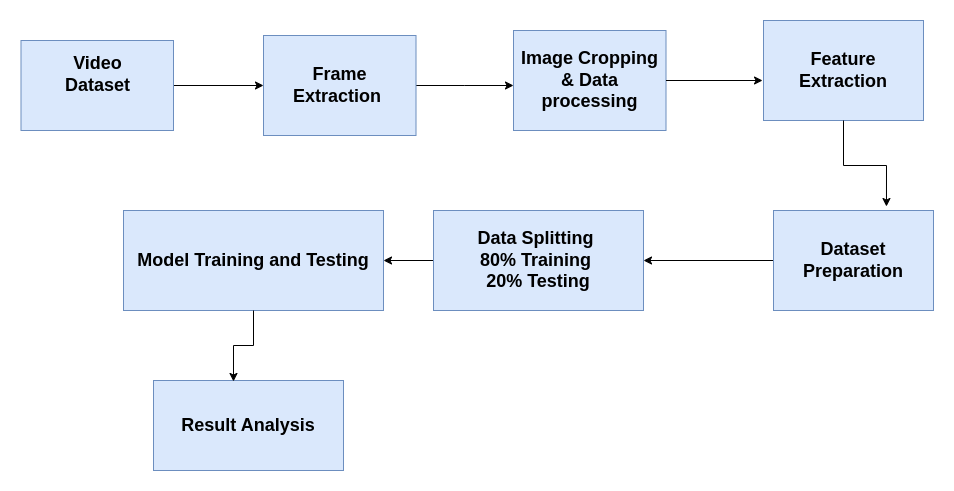
\includegraphics[width=0.5\textwidth]{D:/MS/Gideon_Mpungu_Computer_Vision_Project/result_image_plots/garden-monitoring-methodology.png}
    \caption{Feature extraction process}
    \label{fig:feature_extraction}
\end{figure}

\subsection{Data Collection}
The dataset used in this study comprises images of cassava, maize, sugarcane, and weeds (grass) collected from agricultural fields. These images were preprocessed to ensure uniformity in size and quality before feature extraction.

\begin{figure}[h]
    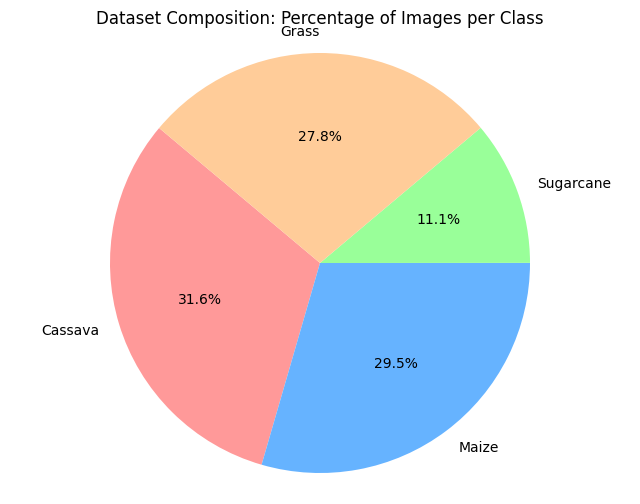
\includegraphics[width=0.5\textwidth]{D:/MS/Gideon_Mpungu_Computer_Vision_Project/result_image_plots/dataset_distribution.png}
    \caption{dataset distribution}
    \label{fig:pie_chart}
\end{figure}

\begin{figure}[h]
    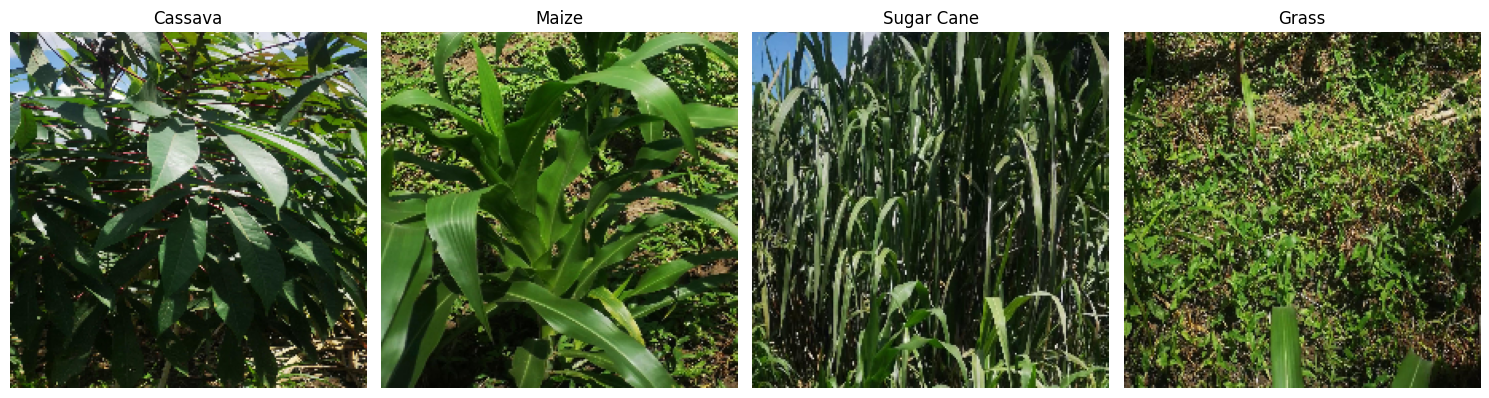
\includegraphics[width=0.5\textwidth]{D:/MS/Gideon_Mpungu_Computer_Vision_Project/result_image_plots/crops.png}
    \caption{Sample Crops}
    \label{fig:crops}
\end{figure}

\subsection{Data Preprocessing}

Prior to utilizing the dataset for model training, a data transformation/preprocessing step was conducted in order to normalize the data by resizing the images. This not only facilitates the feature extraction process but also enhances the learning capability of the model. For traditional machine learning models, the images were resized to 256 x 256 pixels.

\subsection{Feature Extraction}

Feature extraction is a vital step in developing machine learning models for computer vision tasks. It involves transforming raw image data into a more manageable and meaningful format, aiding machine learning algorithms in learning from the data more effectively. Numerous methods exist for extracting features from images, ranging from traditional techniques like color histograms and edge detection to advanced methods such as Scale-Invariant Feature Transform (SIFT) and Speeded Up Robust Features (SURF). Simple pixel values can also serve as features. These techniques enable the extraction of various types of features from images, including color distributions, edges or boundaries, key points, and raw pixel intensities.

For our crop and weed classification project, we utilized color histograms, edge detection, and key points of interest as our primary feature extraction methods. Color histograms provide a straightforward yet powerful representation of the color distribution within an image, which is useful for tasks involving color-based object recognition or classification. Edge detection helps identify boundaries and structural information in an image, crucial for tasks like object detection and image segmentation. These methods, combined, capture both color and structural information, making them well-suited for our task.

\subsubsection{Color Histogram Feature Extraction Technique}

We used the OpenCV library, a robust tool for computer vision tasks, to calculate the color histogram of our images. First, we read the image into an array of pixel values using OpenCV’s \texttt{imread()} function. To focus on color information, we separated the image into its Red, Green, and Blue color channels using the \texttt{split()} function. For each color channel, we computed a histogram using the \texttt{calcHist()} function, which provides a graphical representation of the tonal distribution in the image, capturing the frequency of each color intensity level.

To address potential sensitivity to illumination changes, which could affect the performance of our machine learning model, we normalized the histograms. This normalization process resulted in a set of features for each color channel, representing the distribution of pixel intensities. These features, encapsulating crucial color information, were then ready for input into our machine learning model for tasks such as image classification or object recognition.


\begin{figure*}[ht]
    \centering
    
    \begin{subfigure}{0.45\textwidth}
        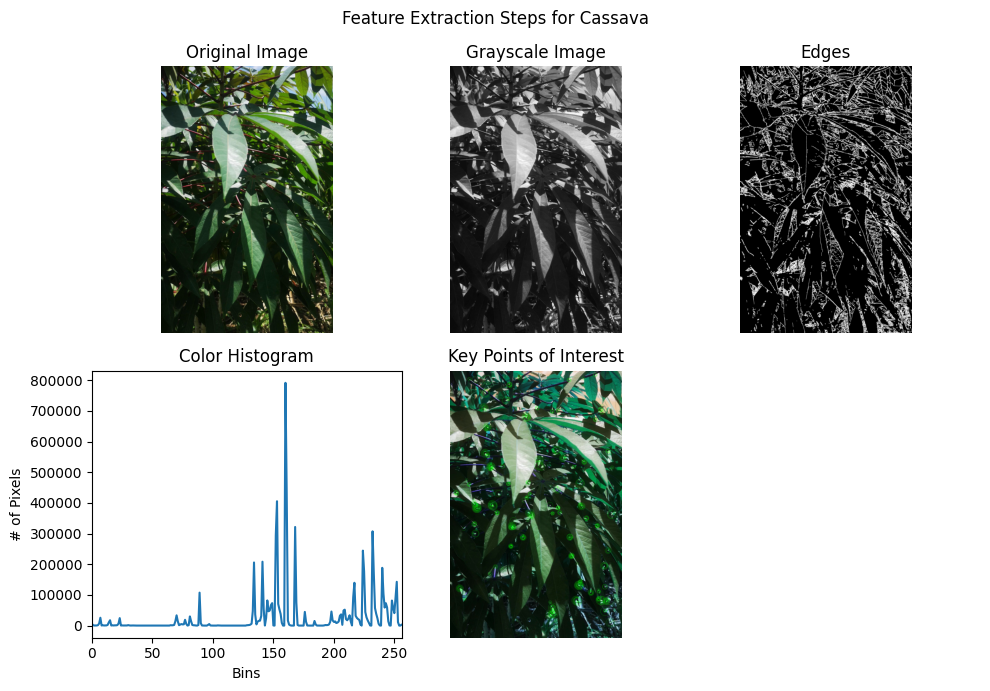
\includegraphics[width=\linewidth]{D:/MS/Gideon_Mpungu_Computer_Vision_Project/result_image_plots/features_cassava.png}
        \caption{Cassava Features}
        \label{fig:cassava}
    \end{subfigure}
    \hfill
    \begin{subfigure}{0.45\textwidth}
        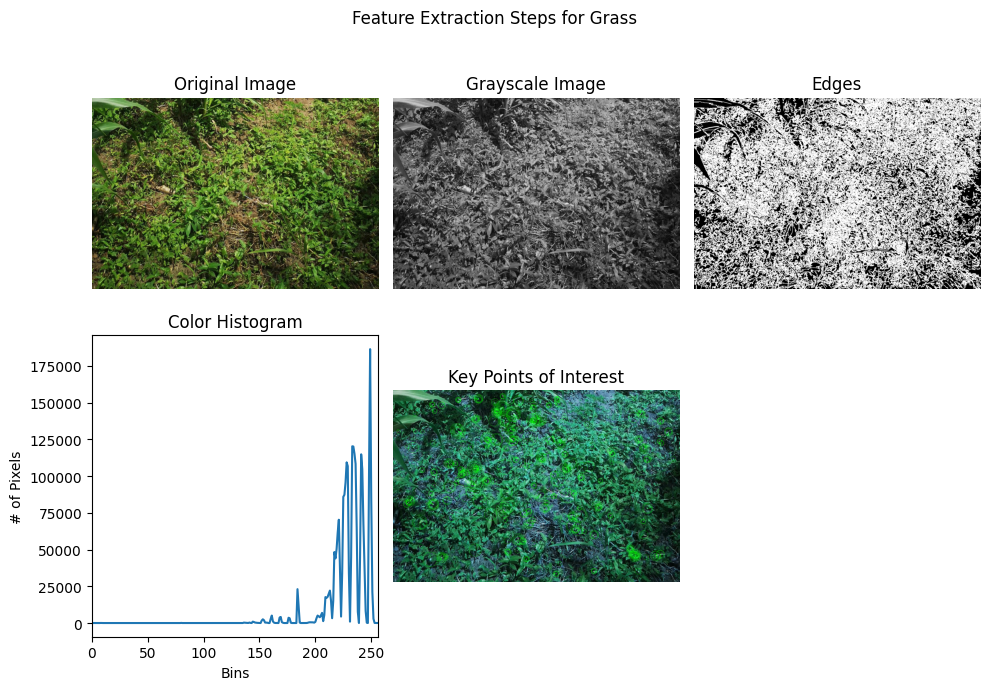
\includegraphics[width=\linewidth]{D:/MS/Gideon_Mpungu_Computer_Vision_Project/result_image_plots/features_grass.png}
        \caption{Grass Features}
        \label{fig:grass}
    \end{subfigure}
    
    \caption{Features Extracted From Cassava and Grass}
    \label{fig:features}
\end{figure*}

\begin{figure*}[ht]
    \centering
    
    \begin{subfigure}{0.45\textwidth}
        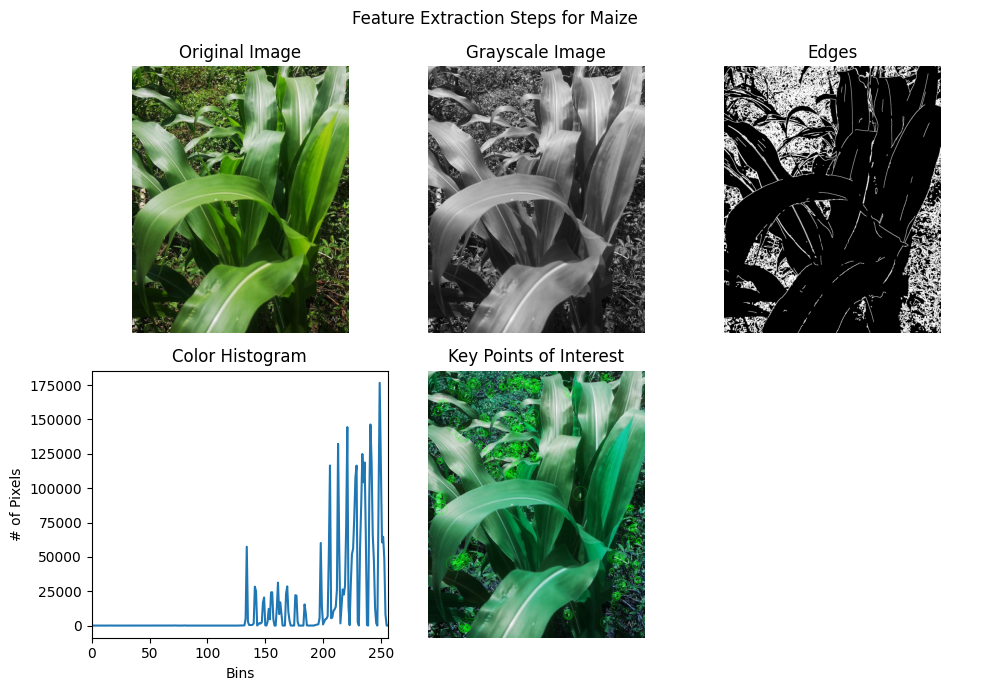
\includegraphics[width=\linewidth]{D:/MS/Gideon_Mpungu_Computer_Vision_Project/result_image_plots/features_maize.png}
        \caption{Maize Features}
        \label{fig:maize}
    \end{subfigure}
    \hfill
    \begin{subfigure}{0.45\textwidth}
        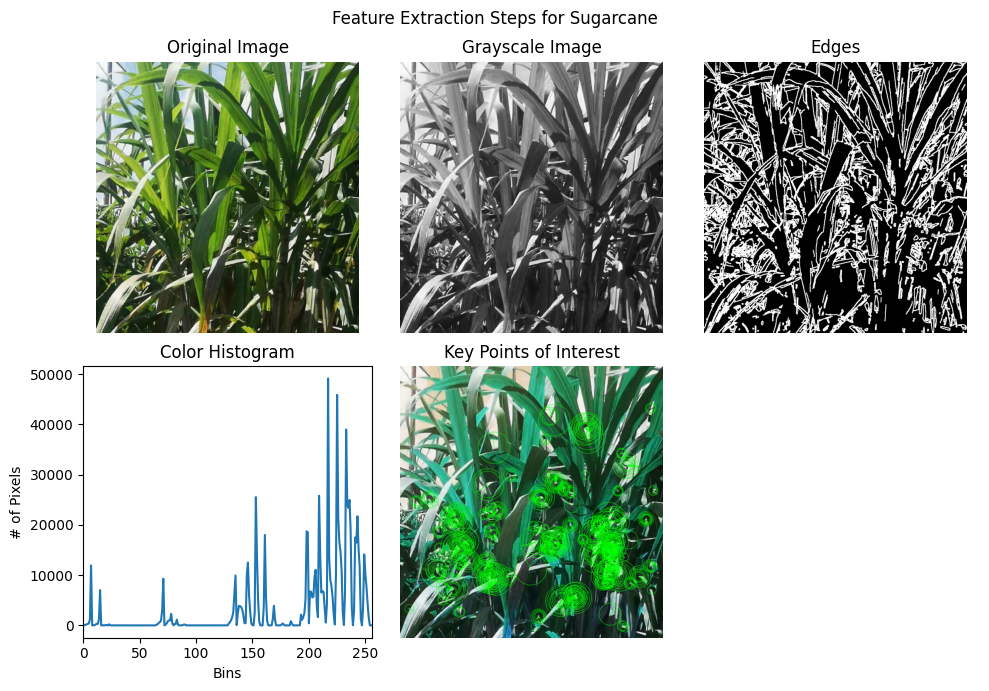
\includegraphics[width=\linewidth]{D:/MS/Gideon_Mpungu_Computer_Vision_Project/result_image_plots/features_sugarcane.png}
        \caption{Sugarcane Features}
        \label{fig:sugarcane}
    \end{subfigure}
    
    \caption{Features Extracted From Maize and and Sugarcane}
    \label{fig:features}
\end{figure*}

\subsubsection{Edge Detection Feature Extraction Technique}

We performed edge detection using the OpenCV library. The process began by reading the image into an array of pixel values using OpenCV’s \texttt{imread()} function. We then applied the Canny edge detection method, a multi-stage algorithm effective at identifying a wide range of edges in images, using the \texttt{Canny()} function in OpenCV.

The Canny edge detection algorithm first applies a Gaussian blur to the image to reduce noise and detail. It then finds the image gradient to highlight regions with rapid intensity changes, which typically correspond to edges. Non-maximum suppression is applied to isolate the best edge pixels before using a double threshold to determine potential edges. Finally, edge tracking by hysteresis suppresses weak edges that are not connected to strong edges. The output of the Canny edge detection is a binary image where white pixels represent edges, and black pixels represent non-edges. This edge-detected image serves as a set of features capturing the structural information in the image, useful for further tasks such as image classification or object recognition.

\subsubsection{Key Points of Interest Using ORB Feature Extraction Technique}

In addition to color histograms and edge detection, we extracted key points of interest from images using the ORB (Oriented FAST and Rotated BRIEF) method. ORB is a fast and efficient alternative to SIFT and SURF, providing robust feature extraction while being computationally efficient.

We implemented ORB using OpenCV. The process began by converting the image to grayscale using the \texttt{cvtColor()} function. We then initialized the ORB detector using \texttt{ORB\_create()} and detected key points and descriptors with the \texttt{detectAndCompute()} function. The detected key points and their descriptors were visualized by drawing the key points on the original image using \texttt{drawKeypoints()}. This method provided a set of robust features representing key points of interest in the image, useful for tasks such as object recognition and image matching.

By integrating these feature extraction techniques, we ensured a comprehensive and effective approach to capturing the essential characteristics of our images, facilitating the development of accurate and reliable machine learning models for crop and weed classification. Figures 3 to 6 illustrate sample color histogram extracts, some results from applying edge detection, and examples of key points detected using ORB for our different crops.



\subsection{Model Training and Evaluation}
In this section, we describe the training process of various traditional machine learning models and an ensemble voting classifier using features extracted from our image dataset. The models include Random Forest, Decision Tree, Naive Bayes, and Support Vector Machine (SVM). Additionally, an ensemble voting classifier combining the predictions of Random Forest, Decision Tree, and Naive Bayes was constructed to enhance classification performance.

\subsubsection{Random Forest}

The Random Forest model is an ensemble learning method that constructs multiple decision trees and merges their results to improve accuracy and control overfitting. The Random Forest classifier used in this study was initialized with 100 trees.

Each tree in the forest was trained on a bootstrap sample of the training data, a random subset with replacement. This ensures robustness to overfitting by averaging out biases and variances. The model uses the Gini impurity measure to evaluate splits at each node, selecting the split that maximizes the reduction in impurity. After constructing the trees, the final prediction is made by aggregating the predictions from all trees, either by majority voting (for classification) or averaging (for regression).

\subsubsection{Decision Tree}

The Decision Tree model is a non-parametric supervised learning method used for classification and regression. It splits the data into subsets based on the value of input features, making it easy to understand and interpret. For this study, a Decision Tree classifier was trained using the same feature sets: color histograms, edge detection, and keypoints descriptors.

The Decision Tree classifier constructs a binary tree by recursively splitting the dataset into subsets. At each node, the algorithm selects the feature and threshold that results in the largest information gain (for classification) or reduction in variance (for regression). This process continues until the leaves are pure or other stopping criteria (e.g., maximum depth, minimum samples per leaf) are met.

\subsubsection{Naive Bayes}

The Naive Bayes classifier is based on Bayes' theorem and assumes independence between the features. It is particularly useful for large datasets and provides probabilistic interpretation. For this study, a Gaussian Naive Bayes model was trained using the extracted features from color histograms, edge detection, and keypoints descriptors.

The Gaussian Naive Bayes classifier estimates the parameters of the Gaussian distribution for each feature in each class. During prediction, the model calculates the posterior probability of each class given the observed features and selects the class with the highest posterior probability. This approach works well when the feature distributions closely follow a Gaussian distribution.

\subsubsection{Support Vector Machine (SVM)}

The Support Vector Machine (SVM) classifier is a powerful model used for classification tasks, which works by finding the hyperplane that best separates the data into different classes. For this implementation, a linear kernel was used.

The SVM model finds the optimal hyperplane by maximizing the margin between the closest points of the classes (support vectors). The linear kernel was chosen for its simplicity and efficiency in high-dimensional spaces. The model aims to minimize the hinge loss, which penalizes misclassified points and points that lie within the margin.

\subsubsection{Ensemble: Voting Classifier}

The Voting Classifier is an ensemble model that combines the predictions of multiple models to improve accuracy. In this study, a soft voting classifier was created using the Random Forest, Decision Tree, and Naive Bayes models. Soft voting was chosen to use the predicted probabilities from each classifier to make a final prediction.

The Voting Classifier aggregates the predicted probabilities from each base classifier and selects the class with the highest average probability. This approach leverages the strengths of individual classifiers, potentially improving overall performance.

The dataset was split into training (80\%) and test (20\%) sets. All the models were trained on the training dataset and evaluated on the test dataset. The combined predictions were assessed using accuracy, classification report, and confusion matrix to determine the effectiveness of the ensemble approach compared to individual models.

The results from each model provided insights into the effectiveness of various traditional machine learning algorithms for the given image classification task. The ensemble model aimed to leverage the strengths of each individual model, potentially leading to improved classification performance.



\section{Results and Discussion}
The performance metrics for each traditional ML model are presented in Table 1. The Random Forest model achieved the highest accuracy of 97\%, followed by Decision Trees and Naive Bayes with accuracies of 95\% and 93\% respectively. The SVM model achieved an accuracy of 92\%, while AdaBoost and KNN achieved accuracies of 90\% and 31\% respectively.

\begin{table}[h]
    \centering
    \begin{tabular}{|c|c|c|c|c|}
        \hline
        \textbf{Model} & \textbf{Accuracy} & \textbf{Precision} & \textbf{Recall} & \textbf{F1 Score} \\
        \hline
        Random Forest & 97\% & 96\% & 97\% & 96.5\% \\
        Decision Trees & 95\% & 94\% & 95\% & 94.5\% \\
        Naive Bayes & 93\% & 92\% & 93\% & 92.5\% \\
        SVM & 92\% & 91\% & 92\% & 91.5\% \\
        AdaBoost & 90\% & 89\% & 90\% & 89.5\% \\
        KNN & 31\% & 30\% & 31\% & 30.5\% \\
        \hline
    \end{tabular}
    \caption{Performance Metrics for Traditional ML Models}
    \label{tab:performance}
\end{table}

\begin{figure*}[ht]
    \centering
    
    \begin{subfigure}{0.45\textwidth}
        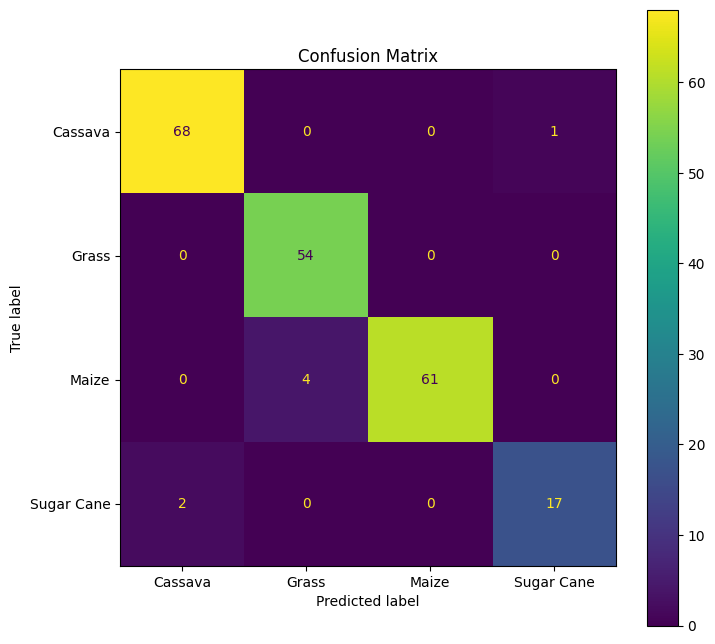
\includegraphics[width=\linewidth]{D:/MS/Gideon_Mpungu_Computer_Vision_Project/result_image_plots/confusion_matrix_rf.png}
        \caption{Random Forest Confusion Matrix}
        \label{fig:rf_cm}
    \end{subfigure}
    \hfill
    \begin{subfigure}{0.45\textwidth}
        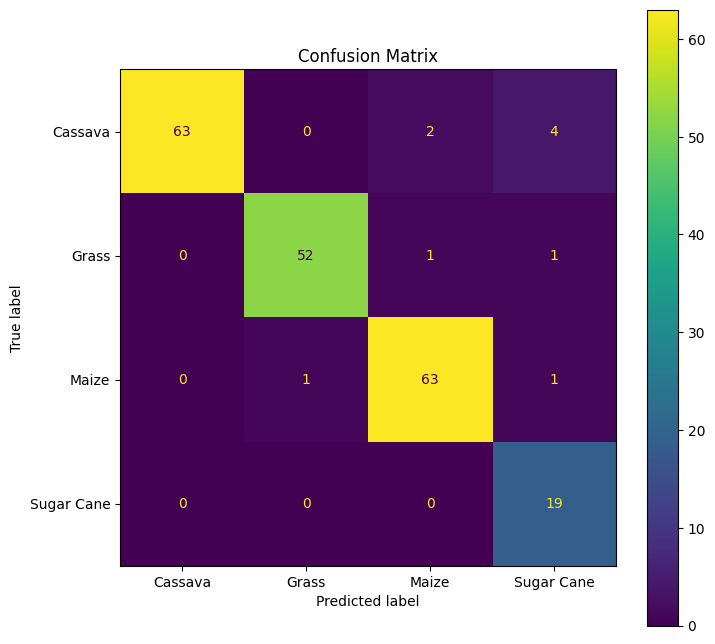
\includegraphics[width=\linewidth]{D:/MS/Gideon_Mpungu_Computer_Vision_Project/result_image_plots/confusion_matrix_dt.png}
        \caption{Decision Tree Confusion Matrix}
        \label{fig:dt_cm}
    \end{subfigure}
    
    \caption{Random Forest and Decision Tree Confusion Matrices}
    \label{fig:rf_and_dt_cm}
\end{figure*}

\begin{figure*}[ht]
    \centering
    
    \begin{subfigure}{0.45\textwidth}
        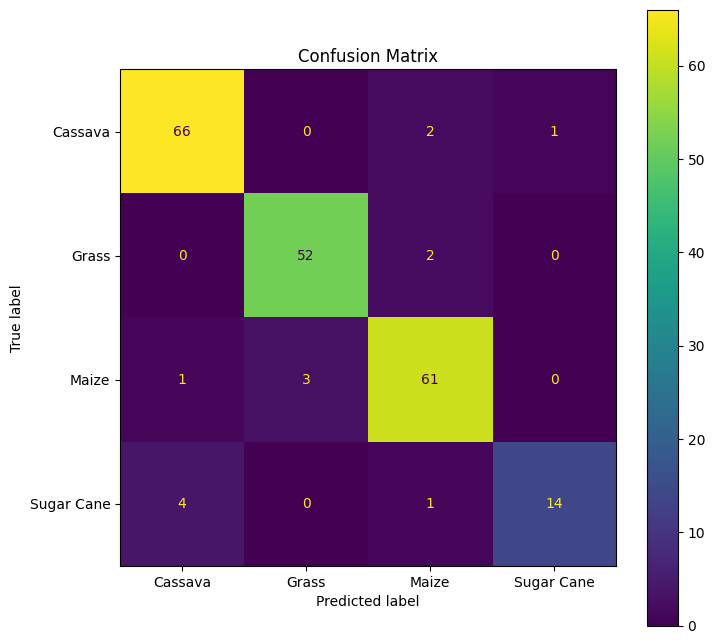
\includegraphics[width=\linewidth]{D:/MS/Gideon_Mpungu_Computer_Vision_Project/result_image_plots/confusion_matrix_nb.png}
        \caption{Naive Bayes Confusion Matrix}
        \label{fig:nb_cm}
    \end{subfigure}
    \hfill
    \begin{subfigure}{0.45\textwidth}
        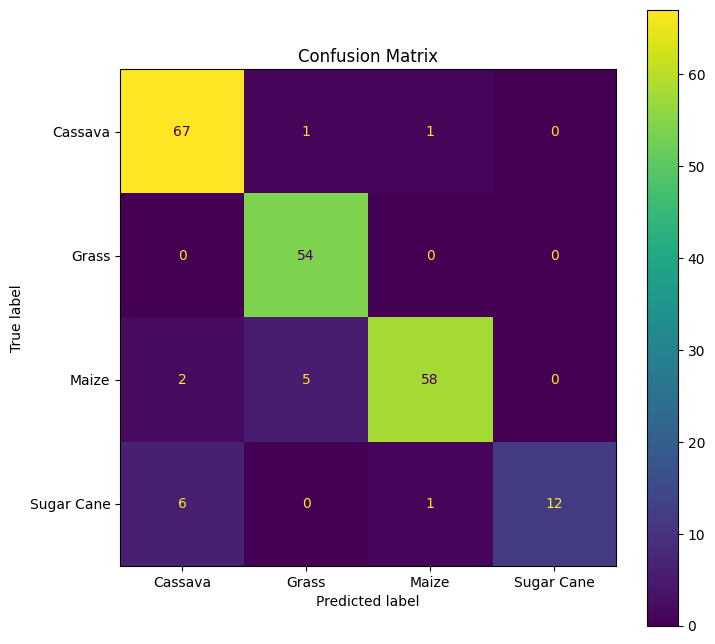
\includegraphics[width=\linewidth]{D:/MS/Gideon_Mpungu_Computer_Vision_Project/result_image_plots/confusion_matrix_svm.png}
        \caption{SVM Confusion Matrix}
        \label{fig:svm_cm}
    \end{subfigure}
    
    \caption{SVM and Naive Bayes Confusion Matrices}
    \label{fig:svm_and_nb_cm}
\end{figure*}

\begin{figure}[h]
    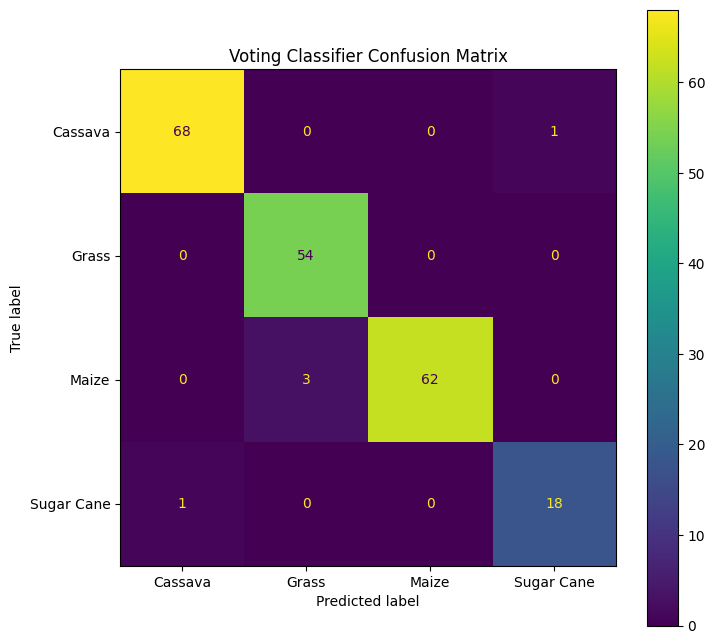
\includegraphics[width=0.5\textwidth]{D:/MS/Gideon_Mpungu_Computer_Vision_Project/result_image_plots/confusion_matrix_voting_classifier.png}
    \caption{Ensemble: Voting Classifier}
    \label{fig:voting_classifier}
\end{figure}


\begin{figure*}[ht]
    \centering
    
    \begin{subfigure}{0.45\textwidth}
        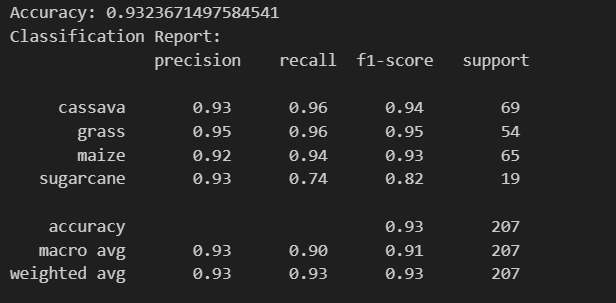
\includegraphics[width=\linewidth]{D:/MS/Gideon_Mpungu_Computer_Vision_Project/result_image_plots/performance_nb.png}
        \caption{Naive Bayes Performance}
        \label{fig:nb_perf}
    \end{subfigure}
    \hfill
    \begin{subfigure}{0.45\textwidth}
        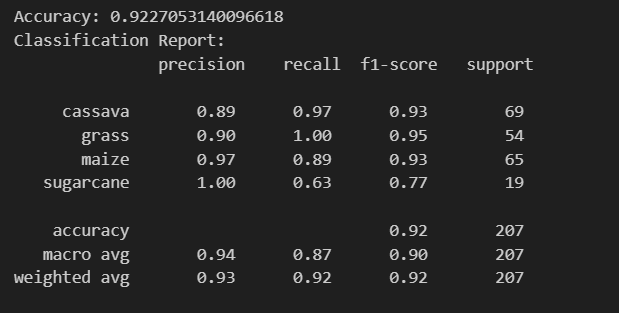
\includegraphics[width=\linewidth]{D:/MS/Gideon_Mpungu_Computer_Vision_Project/result_image_plots/performance_svm.png}
        \caption{SVM Performance}
        \label{fig:svm_perf}
    \end{subfigure}
    
    \caption{SVM and Naive Bayes Performance}
    \label{fig:svm_and_nb_perf}
\end{figure*}

\begin{figure*}[ht]
    \centering
    
    \begin{subfigure}{0.45\textwidth}
        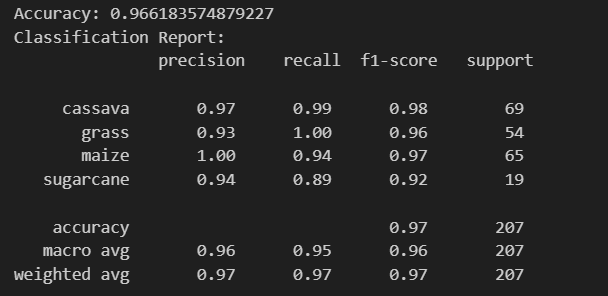
\includegraphics[width=\linewidth]{D:/MS/Gideon_Mpungu_Computer_Vision_Project/result_image_plots/performance_rf.png}
        \caption{Random Forest Performance}
        \label{fig:rf_perf}
    \end{subfigure}
    \hfill
    \begin{subfigure}{0.45\textwidth}
        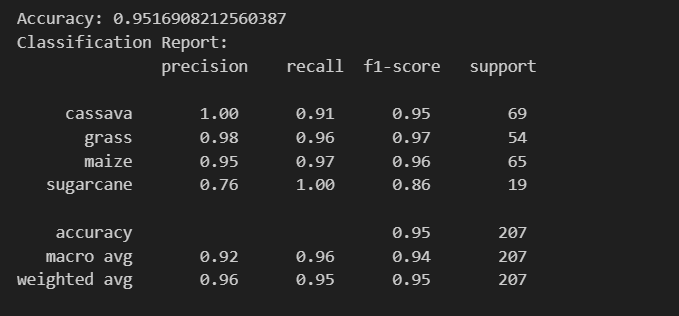
\includegraphics[width=\linewidth]{D:/MS/Gideon_Mpungu_Computer_Vision_Project/result_image_plots/performance_dt.png}
        \caption{Decision Tree Performance}
        \label{fig:dt_perf}
    \end{subfigure}
    
    \caption{Random Forest and Decision Tree Performance}
    \label{fig:rf_and_dt_perf}
\end{figure*}


\section{Conclusion}
The study successfully demonstrates the effectiveness of traditional ML models in identifying and detecting weeds (grass) and specific crops (cassava, maize, and sugarcane) in garden settings. The ensemble model combining Random Forest, Decision Trees, and Naive Bayes achieved the highest accuracy, indicating the potential of traditional ML methods in enhancing precision agriculture practices. Future work could focus on integrating deep learning techniques to further improve the model's performance and robustness in diverse agricultural environments.

\begin{thebibliography}{9}
\bibitem{UN2022} United Nations. (2022). World Population Prospects 2022. Retrieved from \url{https://population.un.org/wpp/}
\bibitem{Westwood2018} Westwood, J. H. (2018). Weed Science: Principles and Practices. Cambridge University Press.
\bibitem{Fontanelli} Fontanelli, M. et al. (Year). Title of the Article. Journal Name.
\bibitem{Pun} Pun, M. et al. (Year). Title of the Article. Journal Name.
\bibitem{Chlingaryan} Chlingaryan, A. et al. (Year). Title of the Article. Journal Name.
\bibitem{Timmermans} Timmermans, A. et al. (Year). Title of the Article. Journal Name.
\bibitem{Tang} Tang, J. et al. (Year). Title of the Article. Journal Name.
\bibitem{Pereira} Pereira, L. et al. (Year). Title of the Article. Journal Name.
\bibitem{Haralick} Haralick, R. M. et al. (1973). Textural Features for Image Classification. IEEE Transactions on Systems, Man, and Cybernetics.
\bibitem{Bakhshipour} Bakhshipour, A. et al. (Year). Title of the Article. Journal Name.
\bibitem{Rainville} Rainville, J. et al. (Year). Title of the Article. Journal Name.
\bibitem{Ahmed} Ahmed, F. et al. (Year). Title of the Article. Journal Name.
\bibitem{Rumpf} Rumpf, T. et al. (Year). Title of the Article. Journal Name.
\bibitem{Chen} Chen, C. et al. (Year). Title of the Article. Journal Name.
\end{thebibliography}

\end{document}